\documentclass[a4paper]{article}

\usepackage[english]{babel}
\usepackage[utf8]{inputenc}
\usepackage{amsmath}
\usepackage{graphicx}
\usepackage[colorinlistoftodos]{todonotes}
\usepackage{amsfonts}
\addtolength{\oddsidemargin}{ 0 in}
\addtolength{\evensidemargin}{ 0 in}
\addtolength{\textwidth}{ 1 in}
\addtolength{\topmargin}{-.875in}
\addtolength{\textheight}{1 in}
\usepackage[all]{xy}
\usepackage{caption}
\usepackage{subcaption}


\title{University of Oslo: Bachelor Project \\ \textbf{RBNS(Reported But Not Settled) Predictions Using Data From an Insurance Company} }

\author{Joël Fomete Tankmo}


\date{\today}


\begin{document}




\maketitle


\newpage


\section{Introduction}

Claims are never settled  immediately, and for some types of injuries or damage, delays are rather long. For non life insurance it is an obligation to set aside technical reserve to settle claims that have occurred in the past calendar years.

A lack of enough reserve can have a direct impact on an insurance company downfall. Downfall that can have a negative effect on policy holders, shareholders and the insurance company employees.     
Between the time that the incident is reported by the customer to the insurance company until the final settlement of the case, there is a delay. An estimate of the payment to be made in the future may therefore affect management, investor and shareholders decision. 

In order to give a realistic financial picture of  all the claims  that are in the process of being liquidated but not finished we need to set up a RBNS-reserve (reported, but not settled) base on the distribution of the amount that will eventually be pay.\\
The paper is set out as follows. In Section 2 we define the notation and describe the data which we will assume is available. In Section 3, the model which we will actually apply is given. We have the conclusion in section 4, the reference in section 5 and in section 6 we have the appendix R-Programs. \\



\section{Data Analysis}


\raggedright The data set contains information from 2354 customers. They are from RBNS-type and come from one of the property insurance companies in Oslo. Each customer is identified by an incident number allocated by the insurance company.   The data is divided into eight categories:   \textit{ incident number, year of incident, delay, number of incidents (0 or 1), estimated compensation when the incident occurred, regress from the company, what was eventually paid and the RBNS reserve put aside by the company}. 
The years the incidents were reported vary between 2003 and 2015 and the maximum number of year it took to cover all the claims is 7 years.


\begin{figure}[h]
  \centering
  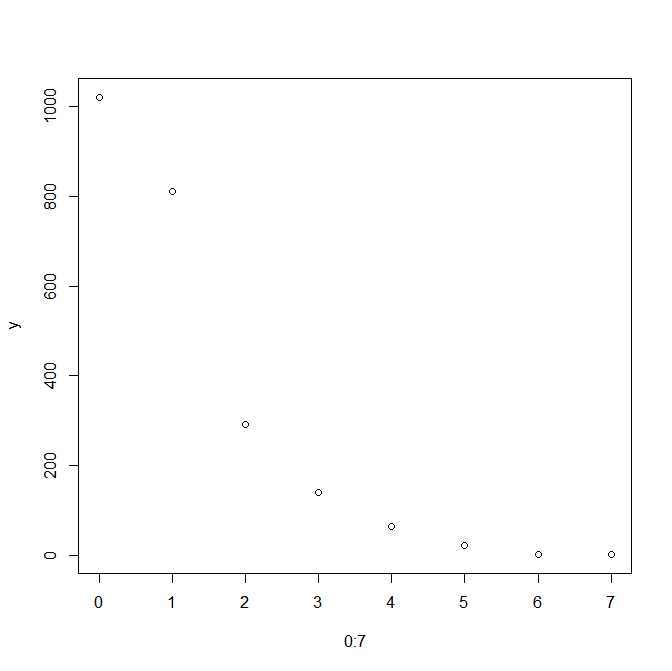
\includegraphics[scale=0.3]{delay.jpg}
  \caption{\textbf{Empirical Distribution of the Delay}}
\end{figure}

\newpage

The scatter-plot of the delay in figure 1 gives us information about the number of claims needed to be settled according to delay. We can see that the graph decreases considerably from the first period to the last period. During the first period we have that 1022 claims were pending versus 1 claim during the last period. That is why the expected delay needed to settled a claim is under 1 year (0.9341546). The number of claims pending during each period is as follow:   1022 ; 811 ; 292 ;141 ; 63  ; 22  ;  2  ;  1.


\begin{figure}[h]
  \centering
  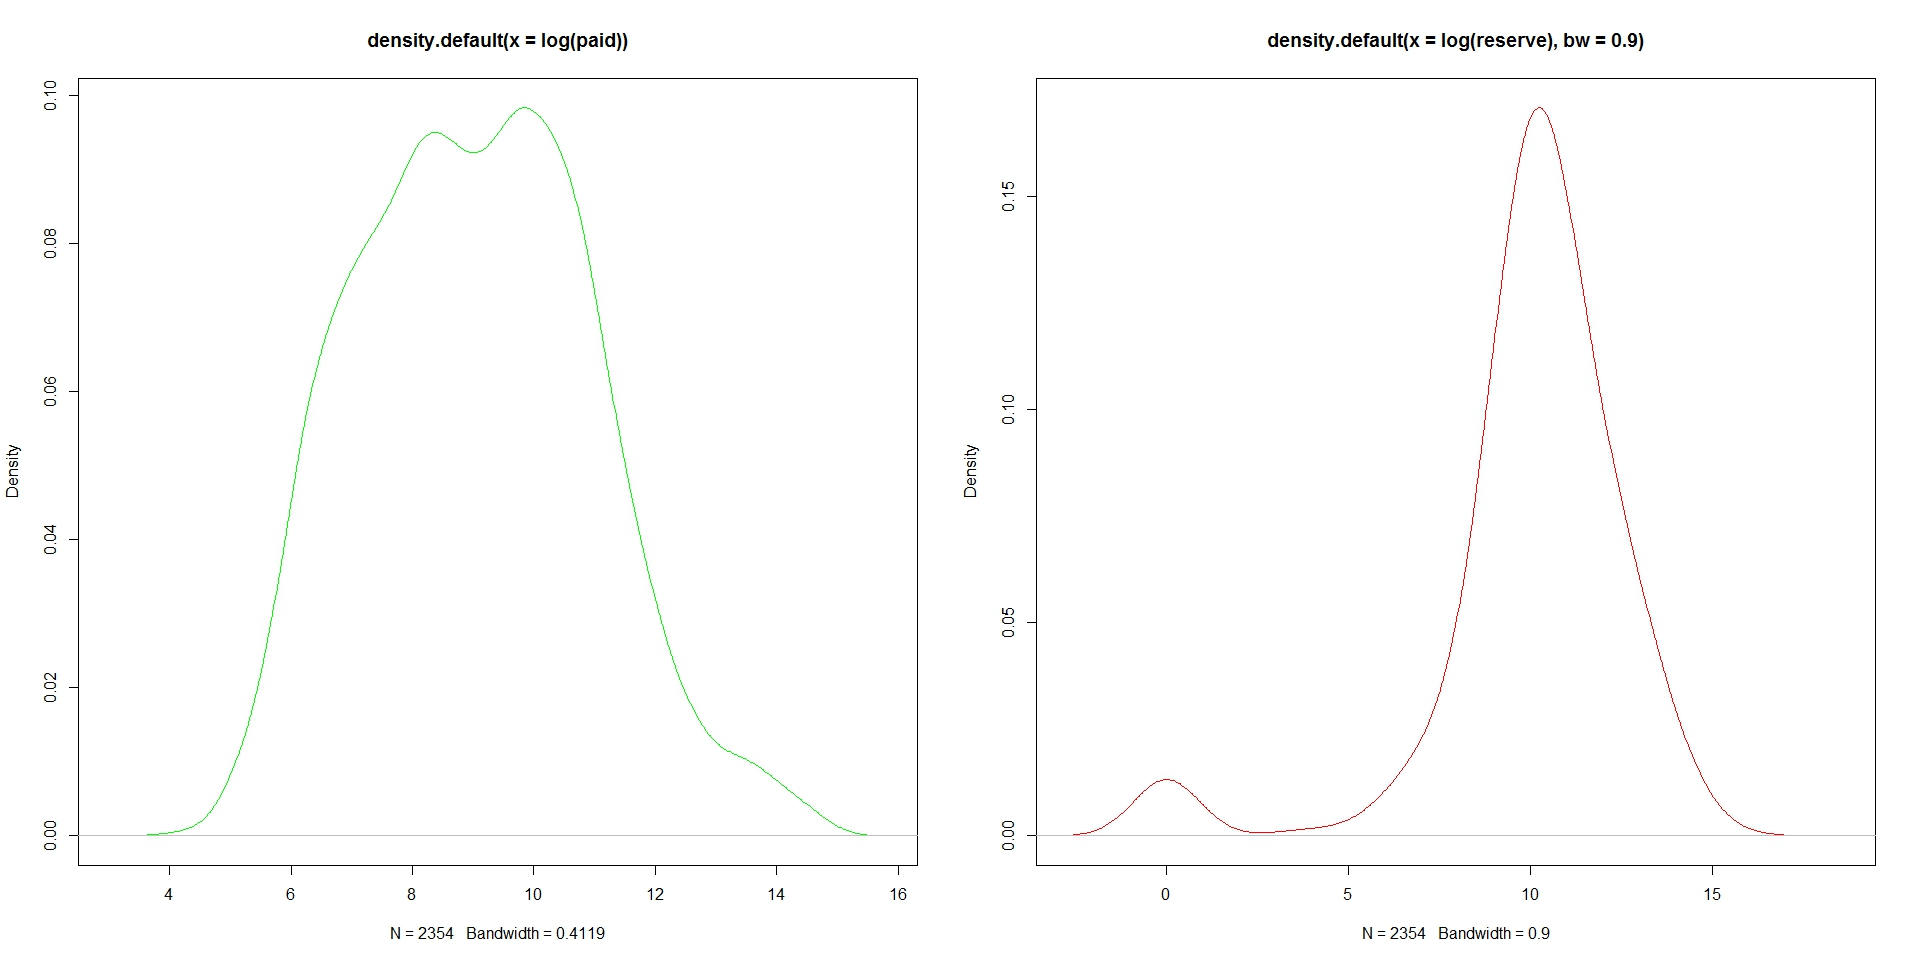
\includegraphics[scale=0.2]{paid_par_reserve.png}
  \caption{\textbf{Distribution of the Logarithm of Paid (left) and RBNS-reserve (right.)}}
\end{figure}

In figure 2, it is not easy to identify the type of distribution. One can see that the stability resulting from a large volume of data produces a rather narrow range . With such stability, in this instance, the log normal distribution approaches the shape of a normal distribution.


\begin{figure}[h]
  \centering
  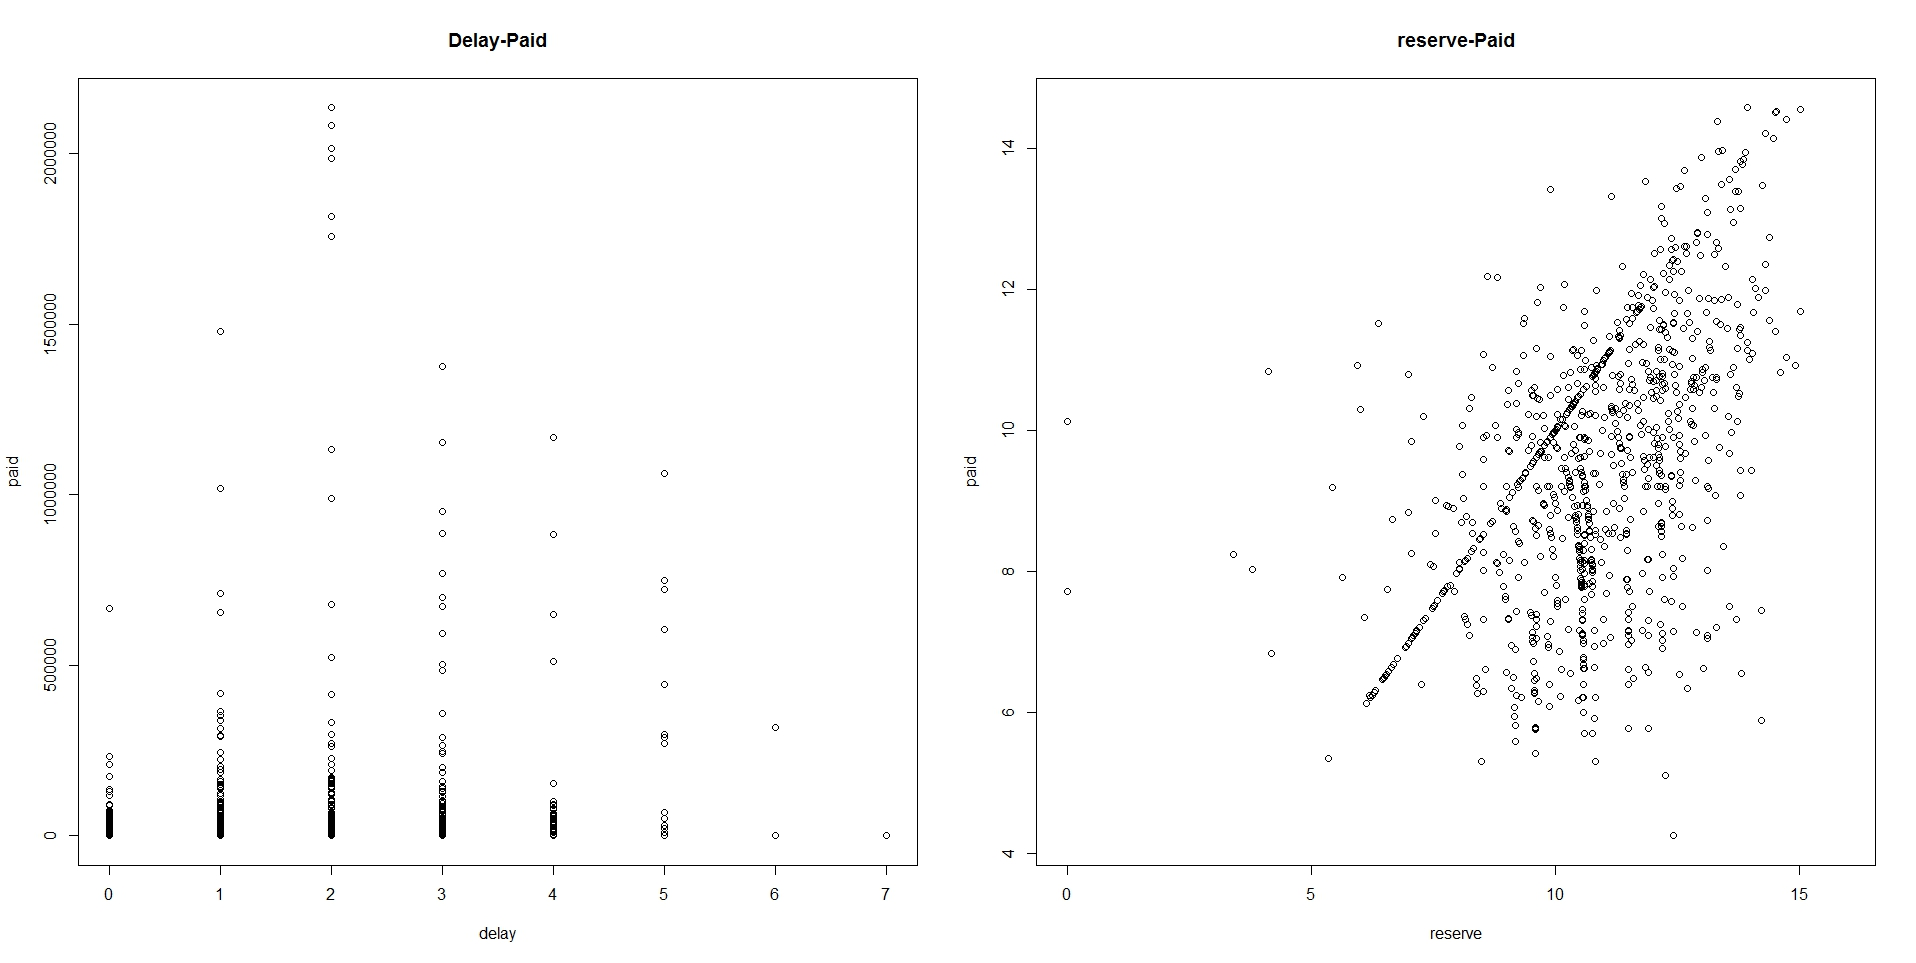
\includegraphics[scale=0.2]{Delay_pay_par_reser_paid.jpeg}
  \caption{\textbf{Delay (left)and RBNS-reserve (right) against final payment.}}
\end{figure}


\newpage

To check if there is a connection between the size of the remunerations and the delay we did in  Figure 3 a scatter plot of the delay against what was paid and a scatter plot of the RBNS reserve agains the delay. We can see that across the entire scatter plot(on the left), there is a huge variation among the data. 
The correlation between the delay and the final payement gave us 0.23 very far from 1. We can therefore say that there is no linear correlation between the delay and the size of the remunerations.\\

The same procedure was made to check if there is a connection between what was paid and the reserve. In the graph on the right we can see that the dots are tightly clustered around a line. The correlation of 0.45 was obtain. We can therefore say that there is a relationship between what was eventually paid and the RBNS-reserve put aside by the company.\\



\begin{figure}[h]
  \centering
  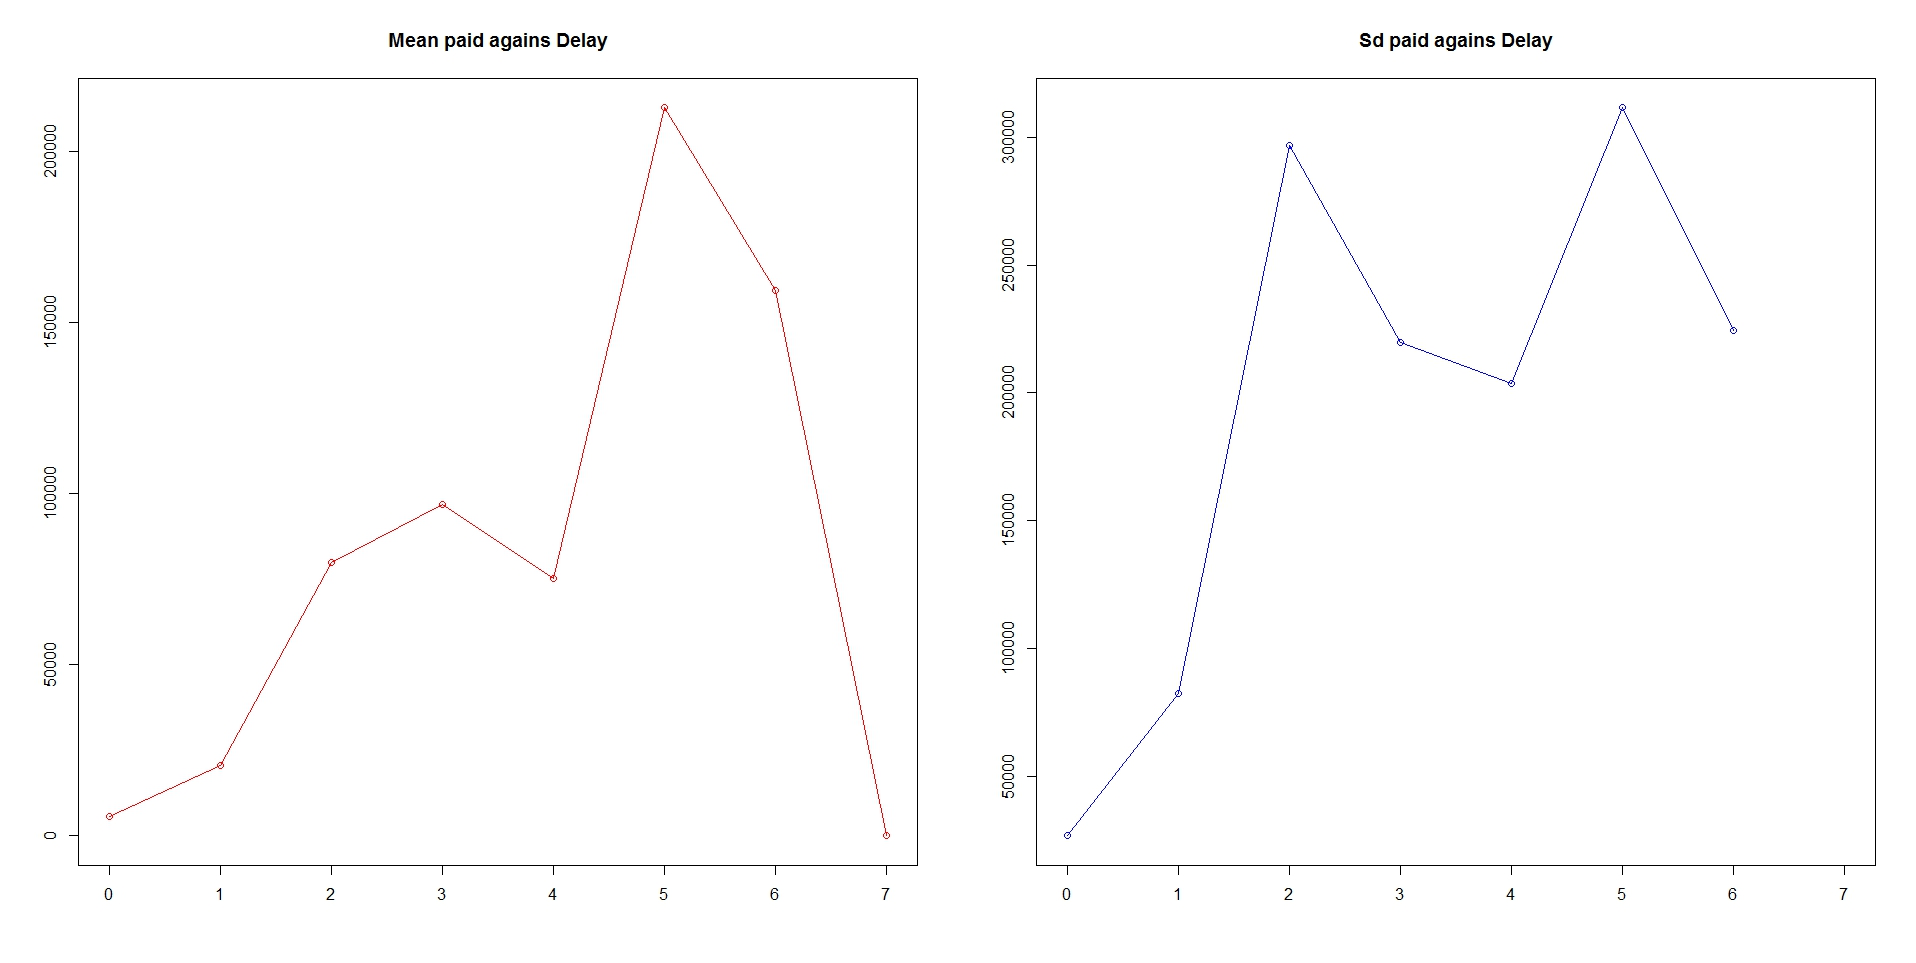
\includegraphics[scale=0.2]{par_Mean_sd_paid_delay.jpeg}
  \caption{\textbf{Mean (left) and standard deviation (right) of final Paid against Delay.}}
\end{figure}


\begin{figure}[h]
  \centering
  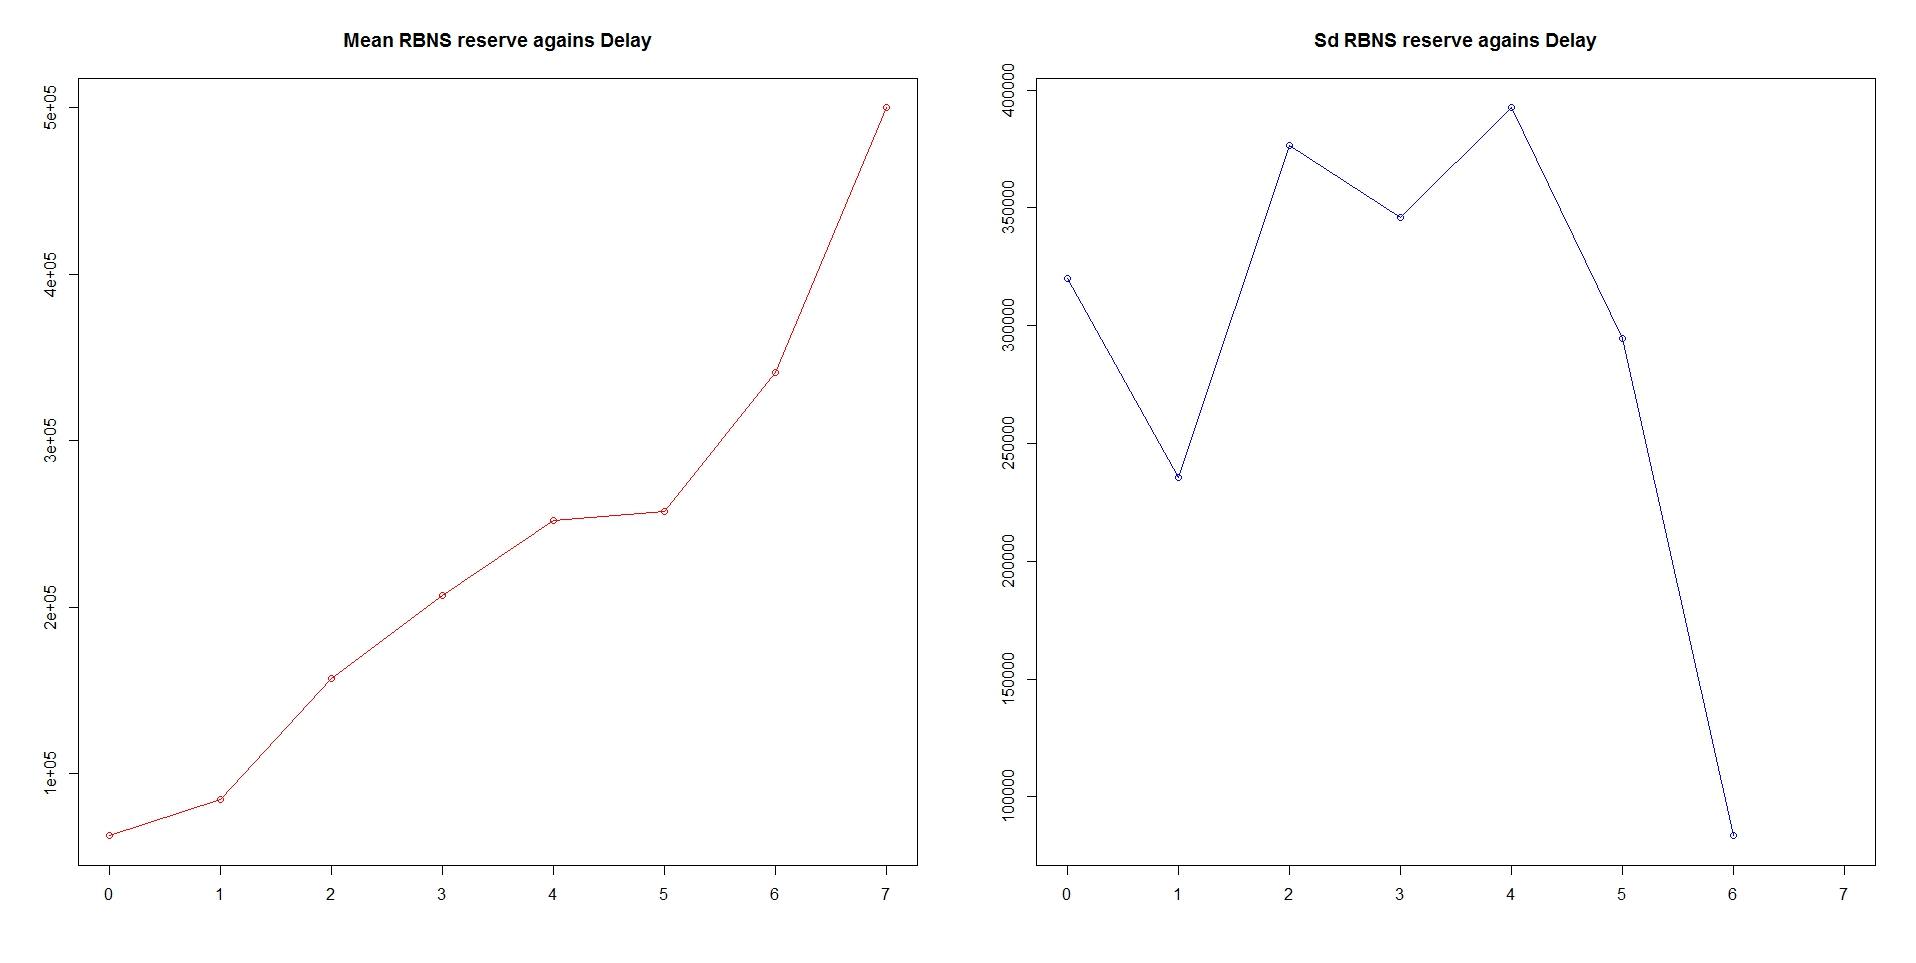
\includegraphics[scale=0.2]{par_mean_sd_reserve_delay.jpeg}
  \caption{\textbf{Mean (left) and standard deviation (right) of RBNS-reserve against Delay}.}
\end{figure}











 \include{table_project.docx}
\textbf{Table 1:   Explanatory variables and descriptive statistics.}
\\


\begin{tabular}{l | p{2.5cm}  p{1.5cm}  p{2cm}}
 ~&Mean &SD\\[.1cm]
\hline \noalign{\smallskip}
Accident year (1=2003; 2=2004; ...; 12=2015) &~~~~~- &~~~~~~-\\[.2cm]
Delay (number of years)&$0.93$    &$ 1.1$\\[.2cm]
Number of incidents: $1$ if an incident occurs; $0$= otherwise &$0.60$ &$    0.49$\\[.2cm]
Estimated compensation when the incident occurred &$57771.96$ &$305401.9$\\[.2cm]
What was eventually paid by the insurance company &$29449.85 $&$140109$\\[.2cm]
The RBNS reserve put aside by the company &$97951.09$ &$309500.2$\\[.1cm] 
\hline  
\end{tabular} \\








 
\textbf{ \\ Table2: Mean and Standard deviation of Paid and RBNS-reserve  according the delay(measure in 1000 NOK)}.\\~\\

\begin{tabular}{| p{2cm }|l| p{1cm}| l | p{1cm}| l | p{1cm}|l | p{1cm}|l | p{1cm} |l |p{1cm} |l |p{1cm}| }
\hline \noalign{\smallskip}
~Delay& year 0& year 1& year2& year3& year4& year5& year6& year7\\[.1cm]
\hline \noalign{\smallskip}
Mean paid  &$5.75$   &$20.69$  & $79.76$  & $96.71$  & $75.30$& $212.73$&$159.31$ &$ 0.00$\\[.2cm]
\hline \noalign{\smallskip}
SD paid &$26.78$&$82.51$&$ 296.60$& $ 219.82$ &$203.62 $& $ 311.48$ &$ 224.32 $&$NA$\\[.2cm]
\hline \noalign{\smallskip}
Mean RBNS & $62.79$ &$ 84.59 $& $157.14$& $ 206.96$&$252.34$&$257.40$&$341.02$&$500.00$\\[.2cm]
\hline \noalign{\smallskip}
SD RBNS &$320.06 $ &$235.51$&$376.63$&$346.06$&$392.44$&$294.47 $&$83.40 $&$NA$\\[.2cm]

\hline 

\end{tabular}



From table 2 we can see that the smallest expected amount that was paid by the insurance company was 5.75 thousand NOK and that was at the beginning. The biggest expected amount paid was for a claim with 6 years of duration and that was 212 thousand NOK.We also observe that the standard or error increase with time. The mean of the RNS reserve put aside by the company increase with the delay. 
In the beginning, the amount that was put aside by the company is 62.79 thousand NOK, After a delay of 7 years the amount is 500 thousand NOK. \\



We have estimated $\alpha$ from the data by using two methods.\\
\textbf{Method 1} :     $\hat\xi_d = z_d  ~~~~~~~~~~~    \hat{\alpha_d} = \frac{\xi^2_d}{Sd^2} $ \\
$ z_d $ is the initial estimates available on the file. \\
With the help of R, we got the following values of alpha for each period of delay:\\

\begin{tabular}{ p{1.5cm} p{1.5cm}  p{1.5cm}  p{1.5cm} p{1.5cm}  p{1.5cm} p{1.5cm} p{1.5cm} } \\
\hline \noalign{\smallskip}
$\alpha_0 $ &$\alpha_1 $ &$\alpha_2 $ &$\alpha_3 $& $\alpha_4 $& $\alpha_5 $& $\alpha_6 $& $\alpha_7$  \\ [.5cm]
$0.05 $ & $0.09$ & $ 0.1 $ & $0.3 $ & $0.6$ & $0.7 $ & $0.4 $ & $3$\\ [.1cm]
\hline   \\

\end{tabular} \\

We can see in the table above that $\alpha$ increases with the period of delay,except for the sixth period where we have 2 claims needed to be settled. The low variation in the beginning is due to the fact that they are many claims needed to be settled.  \\ 



\textbf{Method 2 }:     \begin{align*}E[\sum(n_d - 1) Sd^2] = \sum(n_d - 1)\frac{\xi_d^2}{\alpha}  \\
                \sum(n_d - 1)Sd^2 = (\sum(n_d - 1)\frac{\xi_d^2}{Sd^2}  \\
                 \hat{\alpha} = \frac{\sum(n_d - 1)\xi_d^2}{\sum(n_d - 1)Sd^2}   \\
                  \alpha = 0.606 \\
                  \end{align*} \\
          





Table3: \textbf{Mean and standard variation of the amount paid and the RBNS reserve}. \\~\\

\begin{tabular}{ p{2.5cm} p{2.5cm}  p{2.5cm}  p{2.5cm} p{2.5cm}  p{2.5cm}}
\hline \noalign{\smallskip}
  ~year &Mean paid & SD paid &    Mean RBNS reserve  &  SD RBNS reserve\\[.1cm]
\hline \noalign{\smallskip}   
$2003$&$52295$&  $123846 $&  $193770 $&$ 194586 $\\[.2cm]
$2004$&$19239 $&  $~64766 $&  $~59359 $&  $ ~61811$\\[.2cm]
$2006$&$67521$&  $186350 $& $123393 $&  $145128 $\\[.2cm]
$2007$&$~8222 $& $~25453 $& $~56211 $ & $ 200644 $\\[.2cm]
$2008$&$15657 $& $~62166 $& $101043 $ &$ 298131 $\\[.2cm]
$2009$&$74519 $& $236188 $&$195122 $ &$684771 $\\[.2cm]
$2010$&$34054 $&$156690 $&$ 112983 $&$ 339780 $\\[.2cm]
$2011$&$ 45759 $&$ 161621 $ &$145151 $ &$275433 $\\[.2cm]
$2012$&$30103 $&$ 158217 $ &$102646 $&$281801 $\\[.2cm]
$2013$&$ 22891$&$ 128904  $ &$~71429 $ &$ 235591 $\\[.2cm]
$2014$&$ ~3670 $&$ ~14649  $ &$~26590$ &$~70975 $\\[.2cm]
$2015$&$ ~~260  $&$ ~~1125  $  &$~24763$ &$~38675 $\\[.2cm]
\hline
\end{tabular} \\~\\

From table 2 and 3 we can observe that when the number of claims is high, then there is a better estimation of the mean . This can influence the SD by making it smaller. For example when the delay is 7 we only have one data for it and therefore cannot make a good estimation of either the mean nor the SD.  







 

\section{ RBNS-evaluation with uncertainty} 


The aim here is to develop and implement a Monte Carlo method which returns the distribution of the amount that will be paid. \\

Let J be the  number of incidents needed to be settled in the future, N = 1,...,n\\

The delay d varies between the present value k = 0 and the final value k = 7.   \\
$z_1$,....,$z_n$ are the estimate of the claims that have been delay, we note it $z_d$n .  \\
We have converted the delay vector that were generated into value and we got for each period of delay the following number of claims:\\
1022  811  292  141   63   22    2    1  \\
 

                 
We now assume that  $ \alpha_k  =  \alpha $, that means we assume the variability is the same for all period of delay.\\

$z_1$,....,$z_n$ $\sim$ $z_i$ = $\xi  \times  Y_\alpha$ \\
where E[Y] = 1  and  Y $\sim$ gamma($\alpha$)  \\

E[$z_i$] = $\xi$  and var($z_i$) = $\frac{\xi^2}{\alpha}$ \\  

%$ Y = rgamma\frac{(m,\alpha)}{\alpha}$  \\  
With m = 10 000 simulations we got $\overline{Y} = 1.000946 $ very close to 1.\\
$z_d^* = \xi_d \times Y$



With the help of R we obtained the following values of $z_d^*$, that means the expected amount that the company will eventually  pay in the future period of delay.\\


\begin{tabular}{ p{1.5cm} p{1.5cm}  p{1.5cm}  p{1.5cm} p{1.5cm}  p{1.5cm} p{1.5cm} p{1.5cm} } \\
\hline \noalign{\smallskip}
$z_0^* $ &$z_1^* $ &$z_2^* $ &$z_3^* $& $z_4^* $& $z_5^* $& $z_6^* $& $z_7^*$  \\ [.5cm]
$68205 $ & $87224$ & $ 120559$ & $155902 $ & $228223$ & $242359 $ & $181017 $ & $498104$\\ [.1cm]
\hline   \\

\end{tabular} \\








\begin{figure}[h]
  \centering
  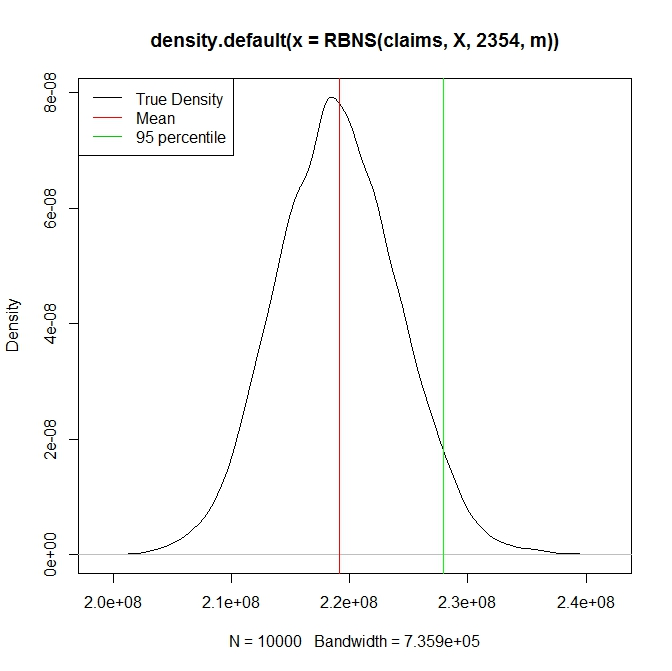
\includegraphics[scale=0.3]{Reserve_RBNS_couleur.jpeg}
  \caption{\textbf{Density function of the RBNS}}
\end{figure}


Figure 6 is the density function of the RBNS with 10000 simulations. The result is a probability distribution showing reserve outcomes at varying probabilities or confidence levels. The result has the shape of a normal (or Gaussian) distribution.The distribution produces a range of possible outcomes.

The statistical mean of this distribution represent the technical reserve that the company will need in order to cover all the claims. A 95\% reserve was obtained, that is the level at which there is 95\% chance that the amount paid by the insurance company will not exceed the estimate. 

The Insurance company may wish to focus on a mean of approximately 219 millions NOK with a standard deviation of  5198190 or error of 2.4\% when deciding for the reserve. If instead of the mean the company choose the 95 percentile, that is 228 millions NOK, there will have an error of 2.3\% which is lower and therefor a lower risk of insolvency. \\




\section{Conclusion} 


The time period between an accident until the compensation is usually very long. As a consequence, the insurer is supposed to calculate the reserve for reported but not settled claims. With the aim of estimating a better reserve, insurers are encouraged  to follow the Solvency II project. The Solvency II Directive (2009/138/EC) is an EU Directive that codifies and harmonises the EU insurance regulation. Primarily this concerns the amount of capital that EU insurance companies must hold to reduce the risk of insolvency.
In a challenging market, which the insurance company faces, there is a necessity to develop more and better models to estimate the RBNS-reserve .
This paper has developed a stochastic framework for claims reserving.
The Method for the RBNS predictions were discussed in this paper, using data from an insurance company. The approach allows for explicit consideration of the random nature of the claims process.  \\



  \textbf{ Acknowledgments.}
The author thanks his supervisor, prof.  Erik Bølviken for valuable comments, remarks and overall help with the research. \\


\section{ References}


- Erik Bølviken (2014) :\textit{Computation and Modelling in Insurance and Finance }


- Peter Dalgaard:\textit{Introductory Statistics with R}


- \textit{$wikipedia.org/wiki/Solvency II Directive$} \\
%http://us.kpmg.com/microsite/FSLibraryDotCom/docs/FRM_QuanUncertainty_WP.pdf

\section{Appendix - R-program}








\begin{verbatim}

Data from the insurance company.
x=read.table('data_mat_stk_project.txt',header=T)$
names(x)
"SkadeNr"       "SkadeAr"       "avvikling"     "antallskader" 
"SkadeEstimat"  "Regress"       "UtbetaltBelop" "RBNS"         
 
Figure 1
delay=x$avvikling
n=length(delay)
mean(x$avvikling)
var(x$avvikling)
sd(x$avvikling)
max(delay)
y=1:8
for (i in y){y[i]=nrow(subset(x,avvikling==(i-1)))}
plot(0:7,y)
#print y to see how many had a delay 0, 1, 2, 3, ...

Figure 2

paid=x$UtbetaltBelop*(-1)
Mean_paid=mean(paid)
sd(paid)
max(paid)
min(paid)
par(mfrow=c(1,2))
plot(density(log(paid)),col="green")

reserve=x$RBNS
reserve_square =reserve^2
reserve=sqrt(reserve_square)
plot(density(log(reserve),bw=0.9),col="red")


Figure 3

# Plot of the delay against what is paid
cor(paid,delay)
#The correlation coefficient of the delay and what was eventually paid is 0.2300282.
#Since it is very small compare to 1, we can conclude that the variables are not positively linearly related. 

par(mfrow=c(1,2))
plot(delay,paid,xlab="delay",ylab="paid",main="Delay-Paid")
# plot reserve against paid

plot(log(reserve),log(paid),xlab="reserve",ylab="paid",main="reserve-Paid")
cor(reserve,paid)

Figure 4

# we plot the mean and sd of paid against delay
paid=x$UtbetaltBelop*(-1)
mean(paid)
paid[x$avvikling==7]
e=rep(0,8)           
for (i in 1:8){e[i]=mean(paid[x$avvikling==i-1])} # we plot the mean of paid again the elements
par(mfrow=c(1,2))
plot(0:7,e,col=2,main="Mean paid agains Delay",type="o",xlab=" ",ylab=" ")

#sum(e)
#sum(paid)
#print e to see what was paid every year

sd(paid)
j=rep(0,8) 
for (i in 1:8){j[i]=sd(paid[x$avvikling==i-1])}
 
plot(0:7,j,col=4,main="Sd paid agains Delay",xlab=" ",ylab=" ",type="o")



Figure 5

# we plot the mean and sd of the reserve again de delay

reserve=x$RBNS
reserve_square =reserve^2
reserve=sqrt(reserve_square)
mean(reserve)
reserve[x$avvikling==7]
e=rep(0,8)          
for (i in 1:8){e[i]=mean(reserve[x$avvikling==i-1])}
par(mfrow=c(1,2))
plot(0:7,e,col=2,main="Mean RBNS reserve agains Delay",type="o",xlab=" ",ylab=" ")
#range(x$RBNS)
sd(reserve)
j=rep(0,8)          
for (i in 1:8){j[i]=sd(reserve[x$avvikling==i-1])}
plot(0:7,j,col=4,main="Sd RBNS reserve against Delay",type="o",xlab=" ",ylab=" ")

#plot(0:7,e,col="red")

We extracted the delay,the year,paid and reserve from the data to build the table.

df=data.frame(year,delay)
aggregate(.~year,data=df,mean)


df=data.frame(year,Reserve)
aggregate(.~year,data=df,mean)


df=data.frame(year,paid)
aggregate(.~year,data=df,sd)


We generated value from the delay vector

y=1:8

for(i in y){y[i]=nrow(subset(x,delay==(i-1)))}
plot(0:7,y)
# 1022  811  292  141   63   22    2    1  claims needed to be settled for each period of the delay
dim(x)=2354
#p_0=1022/2354; p_1=811/2354; p_2=292/2354 ; p_3=141/2354 ; p_4=63/2354 ; p_5=22/2354 ; p_6=2/2354 ; p_7=1/2354
#mysample=sample(c("0year","1year","2year","3year","4year","5year","6year","7year"),10,prob=c(0.4341546,0.34452,0.1240442,0.05989805,0.02676296, 0.009345794,0.0008496177,0.0004248088),replace=T)

p=c(1022,811,292,141,63,22,2,1)/2354
mysample=sample(0:7,2354,prob=p,replace=T)
ant=rep(0,8)
for (i in 1:8){ant[i]=sum(mysample==i-1)}
plot(0:7,ant)
#1028  798  299  137   77   13    2    0   number of incidents (J)that will be settled during each periode of delay(k)

We estimated alfa by two method

methode 1
z=sqrt((x$SkadeEstimat)^2)
var(z)=87948050776
psi=mean(z)

xi_d= rep(0,8)
for(i in 1:8){xi_d[i]=mean(z[delay==(i-1)])}
#### xi_d the the expected compensation for each period of delay
### value of xi_d 
xi_d0=68464.98;xi_d1=87556.20;xi_d2 =121017.62;xi_d3= 156495.39;xi_d4= 229091.47;xi_d5= 243281.62;xi_d6= 181705.50;xi_d7= 500000.00
alfa=xi_d^2/var(z)

alfa0=0.05329798 ; alfa1= 0.0871661; alfa2=  0.1665218; alfa3= 0.278469 ; alfa4= 0.5967489 ; alfa5= 0.6729648 ; alfa6= 0.3754135;   alfa7=  2.842587;

methode 2 # we assume that all the alfa are equall 
expectation=mean(sum(2352-1)*var(z))
expectation=A
A=2.067659e+14
mean(z)=psi
psi=93046.16
B=(sum(2352-1)*psi^2)
B= 2.035399e+13
alfa=B/A
alfa = 0.6059003


We do the following to obtain the reserve.

m=100000
y=rgamma(m,alfa)/alfa
mean(y) #
alfa=1.000946

xi_d=c(68464.98,87556.20,121017.62, 156495.39,229091.47,243281.62,181705.50,500000.00)
z_d=1:8
for(i in 1:8){ z_d[i]=mean(y)*xi_d[i]}
### z_d the expected compensation for each periode of delay tomorrow . z_d= xi_d*mean(y)
### z_d: 68393.03  87464.18 120890.44 156330.92 228850.71 243025.95  181514.54 499474.53
m=10000
N[0]=2354 # number of claims to be settled
#p=c(1028 , 798 , 299 , 137 ,  77 ,  13   , 2   ,0 )/2354
p=c(1022,811,292,141,63,22,2,1)/2354
X=0:7
#N_d=number of delay of length d
claims=c(1022,811,292,141,63,22,2,1)
RBNS=function(claims,X,N0=2354,m){
  rbns=rep(0,m)
  p=claims/2354
  for(i in 1:m){
    D=sample(X,N0,replace=T,prob=p)
    N=rep(0,8)
    for(d in 1:8){
      N[d]=sum(D==(d-1))
      z_d=sum(rgamma(N[d],alfa)/alfa)*xi_d[d]
      rbns[i]=rbns[i]+z_d
      
      }
   }
return(rbns)   }


head(RBNS(claims,X,2354,m)) #  218175104 209596859 2155
e=0.05
reserve = sort(RBNS(claims,X,2354,m))[m*(1-e)]
plot(density(RBNS(claims,X,2354,m)))
abline(v=219090529,col="red")
abline(v=227909617,col="green")
legend("topleft",c("True Density","Mean","95 percentile"),lty=1,col=1:3)

z_d #  68205.39  87224.23 120558.78 155902.03 228222.86 242359.21 181016.55 498104.23 ...

mean(RBNS(claims,X,2354,m))# 219082571 #  by repeating the above described procedure a large number of times and taking the mean of the empirical result, we obtain the reserve 

var(RBNS(claims,X,2354,m)) # 4.247832e+13

sd(RBNS(claims,X,2354,m))  # 6498224




\end{verbatim}




\end{document}


















 
































